
% Default to the notebook output style

    


% Inherit from the specified cell style.




    
\documentclass[11pt]{article}

    
    
    \usepackage[T1]{fontenc}
    % Nicer default font (+ math font) than Computer Modern for most use cases
    \usepackage{mathpazo}

    % Basic figure setup, for now with no caption control since it's done
    % automatically by Pandoc (which extracts ![](path) syntax from Markdown).
    \usepackage{graphicx}
    % We will generate all images so they have a width \maxwidth. This means
    % that they will get their normal width if they fit onto the page, but
    % are scaled down if they would overflow the margins.
    \makeatletter
    \def\maxwidth{\ifdim\Gin@nat@width>\linewidth\linewidth
    \else\Gin@nat@width\fi}
    \makeatother
    \let\Oldincludegraphics\includegraphics
    % Set max figure width to be 80% of text width, for now hardcoded.
    \renewcommand{\includegraphics}[1]{\Oldincludegraphics[width=.8\maxwidth]{#1}}
    % Ensure that by default, figures have no caption (until we provide a
    % proper Figure object with a Caption API and a way to capture that
    % in the conversion process - todo).
    \usepackage{caption}
    \DeclareCaptionLabelFormat{nolabel}{}
    \captionsetup{labelformat=nolabel}

    \usepackage{adjustbox} % Used to constrain images to a maximum size 
    \usepackage{xcolor} % Allow colors to be defined
    \usepackage{enumerate} % Needed for markdown enumerations to work
    \usepackage{geometry} % Used to adjust the document margins
    \usepackage{amsmath} % Equations
    \usepackage{amssymb} % Equations
    \usepackage{textcomp} % defines textquotesingle
    % Hack from http://tex.stackexchange.com/a/47451/13684:
    \AtBeginDocument{%
        \def\PYZsq{\textquotesingle}% Upright quotes in Pygmentized code
    }
    \usepackage{upquote} % Upright quotes for verbatim code
    \usepackage{eurosym} % defines \euro
    \usepackage[mathletters]{ucs} % Extended unicode (utf-8) support
    \usepackage[utf8x]{inputenc} % Allow utf-8 characters in the tex document
    \usepackage{fancyvrb} % verbatim replacement that allows latex
    \usepackage{grffile} % extends the file name processing of package graphics 
                         % to support a larger range 
    % The hyperref package gives us a pdf with properly built
    % internal navigation ('pdf bookmarks' for the table of contents,
    % internal cross-reference links, web links for URLs, etc.)
    \usepackage{hyperref}
    \usepackage{longtable} % longtable support required by pandoc >1.10
    \usepackage{booktabs}  % table support for pandoc > 1.12.2
    \usepackage[inline]{enumitem} % IRkernel/repr support (it uses the enumerate* environment)
    \usepackage[normalem]{ulem} % ulem is needed to support strikethroughs (\sout)
                                % normalem makes italics be italics, not underlines
    

    
    
    % Colors for the hyperref package
    \definecolor{urlcolor}{rgb}{0,.145,.698}
    \definecolor{linkcolor}{rgb}{.71,0.21,0.01}
    \definecolor{citecolor}{rgb}{.12,.54,.11}

    % ANSI colors
    \definecolor{ansi-black}{HTML}{3E424D}
    \definecolor{ansi-black-intense}{HTML}{282C36}
    \definecolor{ansi-red}{HTML}{E75C58}
    \definecolor{ansi-red-intense}{HTML}{B22B31}
    \definecolor{ansi-green}{HTML}{00A250}
    \definecolor{ansi-green-intense}{HTML}{007427}
    \definecolor{ansi-yellow}{HTML}{DDB62B}
    \definecolor{ansi-yellow-intense}{HTML}{B27D12}
    \definecolor{ansi-blue}{HTML}{208FFB}
    \definecolor{ansi-blue-intense}{HTML}{0065CA}
    \definecolor{ansi-magenta}{HTML}{D160C4}
    \definecolor{ansi-magenta-intense}{HTML}{A03196}
    \definecolor{ansi-cyan}{HTML}{60C6C8}
    \definecolor{ansi-cyan-intense}{HTML}{258F8F}
    \definecolor{ansi-white}{HTML}{C5C1B4}
    \definecolor{ansi-white-intense}{HTML}{A1A6B2}

    % commands and environments needed by pandoc snippets
    % extracted from the output of `pandoc -s`
    \providecommand{\tightlist}{%
      \setlength{\itemsep}{0pt}\setlength{\parskip}{0pt}}
    \DefineVerbatimEnvironment{Highlighting}{Verbatim}{commandchars=\\\{\}}
    % Add ',fontsize=\small' for more characters per line
    \newenvironment{Shaded}{}{}
    \newcommand{\KeywordTok}[1]{\textcolor[rgb]{0.00,0.44,0.13}{\textbf{{#1}}}}
    \newcommand{\DataTypeTok}[1]{\textcolor[rgb]{0.56,0.13,0.00}{{#1}}}
    \newcommand{\DecValTok}[1]{\textcolor[rgb]{0.25,0.63,0.44}{{#1}}}
    \newcommand{\BaseNTok}[1]{\textcolor[rgb]{0.25,0.63,0.44}{{#1}}}
    \newcommand{\FloatTok}[1]{\textcolor[rgb]{0.25,0.63,0.44}{{#1}}}
    \newcommand{\CharTok}[1]{\textcolor[rgb]{0.25,0.44,0.63}{{#1}}}
    \newcommand{\StringTok}[1]{\textcolor[rgb]{0.25,0.44,0.63}{{#1}}}
    \newcommand{\CommentTok}[1]{\textcolor[rgb]{0.38,0.63,0.69}{\textit{{#1}}}}
    \newcommand{\OtherTok}[1]{\textcolor[rgb]{0.00,0.44,0.13}{{#1}}}
    \newcommand{\AlertTok}[1]{\textcolor[rgb]{1.00,0.00,0.00}{\textbf{{#1}}}}
    \newcommand{\FunctionTok}[1]{\textcolor[rgb]{0.02,0.16,0.49}{{#1}}}
    \newcommand{\RegionMarkerTok}[1]{{#1}}
    \newcommand{\ErrorTok}[1]{\textcolor[rgb]{1.00,0.00,0.00}{\textbf{{#1}}}}
    \newcommand{\NormalTok}[1]{{#1}}
    
    % Additional commands for more recent versions of Pandoc
    \newcommand{\ConstantTok}[1]{\textcolor[rgb]{0.53,0.00,0.00}{{#1}}}
    \newcommand{\SpecialCharTok}[1]{\textcolor[rgb]{0.25,0.44,0.63}{{#1}}}
    \newcommand{\VerbatimStringTok}[1]{\textcolor[rgb]{0.25,0.44,0.63}{{#1}}}
    \newcommand{\SpecialStringTok}[1]{\textcolor[rgb]{0.73,0.40,0.53}{{#1}}}
    \newcommand{\ImportTok}[1]{{#1}}
    \newcommand{\DocumentationTok}[1]{\textcolor[rgb]{0.73,0.13,0.13}{\textit{{#1}}}}
    \newcommand{\AnnotationTok}[1]{\textcolor[rgb]{0.38,0.63,0.69}{\textbf{\textit{{#1}}}}}
    \newcommand{\CommentVarTok}[1]{\textcolor[rgb]{0.38,0.63,0.69}{\textbf{\textit{{#1}}}}}
    \newcommand{\VariableTok}[1]{\textcolor[rgb]{0.10,0.09,0.49}{{#1}}}
    \newcommand{\ControlFlowTok}[1]{\textcolor[rgb]{0.00,0.44,0.13}{\textbf{{#1}}}}
    \newcommand{\OperatorTok}[1]{\textcolor[rgb]{0.40,0.40,0.40}{{#1}}}
    \newcommand{\BuiltInTok}[1]{{#1}}
    \newcommand{\ExtensionTok}[1]{{#1}}
    \newcommand{\PreprocessorTok}[1]{\textcolor[rgb]{0.74,0.48,0.00}{{#1}}}
    \newcommand{\AttributeTok}[1]{\textcolor[rgb]{0.49,0.56,0.16}{{#1}}}
    \newcommand{\InformationTok}[1]{\textcolor[rgb]{0.38,0.63,0.69}{\textbf{\textit{{#1}}}}}
    \newcommand{\WarningTok}[1]{\textcolor[rgb]{0.38,0.63,0.69}{\textbf{\textit{{#1}}}}}
    
    
    % Define a nice break command that doesn't care if a line doesn't already
    % exist.
    \def\br{\hspace*{\fill} \\* }
    % Math Jax compatability definitions
    \def\gt{>}
    \def\lt{<}
    % Document parameters
    \title{Build a Stock Price Predictor}
    
    
    

    % Pygments definitions
    
\makeatletter
\def\PY@reset{\let\PY@it=\relax \let\PY@bf=\relax%
    \let\PY@ul=\relax \let\PY@tc=\relax%
    \let\PY@bc=\relax \let\PY@ff=\relax}
\def\PY@tok#1{\csname PY@tok@#1\endcsname}
\def\PY@toks#1+{\ifx\relax#1\empty\else%
    \PY@tok{#1}\expandafter\PY@toks\fi}
\def\PY@do#1{\PY@bc{\PY@tc{\PY@ul{%
    \PY@it{\PY@bf{\PY@ff{#1}}}}}}}
\def\PY#1#2{\PY@reset\PY@toks#1+\relax+\PY@do{#2}}

\expandafter\def\csname PY@tok@w\endcsname{\def\PY@tc##1{\textcolor[rgb]{0.73,0.73,0.73}{##1}}}
\expandafter\def\csname PY@tok@c\endcsname{\let\PY@it=\textit\def\PY@tc##1{\textcolor[rgb]{0.25,0.50,0.50}{##1}}}
\expandafter\def\csname PY@tok@cp\endcsname{\def\PY@tc##1{\textcolor[rgb]{0.74,0.48,0.00}{##1}}}
\expandafter\def\csname PY@tok@k\endcsname{\let\PY@bf=\textbf\def\PY@tc##1{\textcolor[rgb]{0.00,0.50,0.00}{##1}}}
\expandafter\def\csname PY@tok@kp\endcsname{\def\PY@tc##1{\textcolor[rgb]{0.00,0.50,0.00}{##1}}}
\expandafter\def\csname PY@tok@kt\endcsname{\def\PY@tc##1{\textcolor[rgb]{0.69,0.00,0.25}{##1}}}
\expandafter\def\csname PY@tok@o\endcsname{\def\PY@tc##1{\textcolor[rgb]{0.40,0.40,0.40}{##1}}}
\expandafter\def\csname PY@tok@ow\endcsname{\let\PY@bf=\textbf\def\PY@tc##1{\textcolor[rgb]{0.67,0.13,1.00}{##1}}}
\expandafter\def\csname PY@tok@nb\endcsname{\def\PY@tc##1{\textcolor[rgb]{0.00,0.50,0.00}{##1}}}
\expandafter\def\csname PY@tok@nf\endcsname{\def\PY@tc##1{\textcolor[rgb]{0.00,0.00,1.00}{##1}}}
\expandafter\def\csname PY@tok@nc\endcsname{\let\PY@bf=\textbf\def\PY@tc##1{\textcolor[rgb]{0.00,0.00,1.00}{##1}}}
\expandafter\def\csname PY@tok@nn\endcsname{\let\PY@bf=\textbf\def\PY@tc##1{\textcolor[rgb]{0.00,0.00,1.00}{##1}}}
\expandafter\def\csname PY@tok@ne\endcsname{\let\PY@bf=\textbf\def\PY@tc##1{\textcolor[rgb]{0.82,0.25,0.23}{##1}}}
\expandafter\def\csname PY@tok@nv\endcsname{\def\PY@tc##1{\textcolor[rgb]{0.10,0.09,0.49}{##1}}}
\expandafter\def\csname PY@tok@no\endcsname{\def\PY@tc##1{\textcolor[rgb]{0.53,0.00,0.00}{##1}}}
\expandafter\def\csname PY@tok@nl\endcsname{\def\PY@tc##1{\textcolor[rgb]{0.63,0.63,0.00}{##1}}}
\expandafter\def\csname PY@tok@ni\endcsname{\let\PY@bf=\textbf\def\PY@tc##1{\textcolor[rgb]{0.60,0.60,0.60}{##1}}}
\expandafter\def\csname PY@tok@na\endcsname{\def\PY@tc##1{\textcolor[rgb]{0.49,0.56,0.16}{##1}}}
\expandafter\def\csname PY@tok@nt\endcsname{\let\PY@bf=\textbf\def\PY@tc##1{\textcolor[rgb]{0.00,0.50,0.00}{##1}}}
\expandafter\def\csname PY@tok@nd\endcsname{\def\PY@tc##1{\textcolor[rgb]{0.67,0.13,1.00}{##1}}}
\expandafter\def\csname PY@tok@s\endcsname{\def\PY@tc##1{\textcolor[rgb]{0.73,0.13,0.13}{##1}}}
\expandafter\def\csname PY@tok@sd\endcsname{\let\PY@it=\textit\def\PY@tc##1{\textcolor[rgb]{0.73,0.13,0.13}{##1}}}
\expandafter\def\csname PY@tok@si\endcsname{\let\PY@bf=\textbf\def\PY@tc##1{\textcolor[rgb]{0.73,0.40,0.53}{##1}}}
\expandafter\def\csname PY@tok@se\endcsname{\let\PY@bf=\textbf\def\PY@tc##1{\textcolor[rgb]{0.73,0.40,0.13}{##1}}}
\expandafter\def\csname PY@tok@sr\endcsname{\def\PY@tc##1{\textcolor[rgb]{0.73,0.40,0.53}{##1}}}
\expandafter\def\csname PY@tok@ss\endcsname{\def\PY@tc##1{\textcolor[rgb]{0.10,0.09,0.49}{##1}}}
\expandafter\def\csname PY@tok@sx\endcsname{\def\PY@tc##1{\textcolor[rgb]{0.00,0.50,0.00}{##1}}}
\expandafter\def\csname PY@tok@m\endcsname{\def\PY@tc##1{\textcolor[rgb]{0.40,0.40,0.40}{##1}}}
\expandafter\def\csname PY@tok@gh\endcsname{\let\PY@bf=\textbf\def\PY@tc##1{\textcolor[rgb]{0.00,0.00,0.50}{##1}}}
\expandafter\def\csname PY@tok@gu\endcsname{\let\PY@bf=\textbf\def\PY@tc##1{\textcolor[rgb]{0.50,0.00,0.50}{##1}}}
\expandafter\def\csname PY@tok@gd\endcsname{\def\PY@tc##1{\textcolor[rgb]{0.63,0.00,0.00}{##1}}}
\expandafter\def\csname PY@tok@gi\endcsname{\def\PY@tc##1{\textcolor[rgb]{0.00,0.63,0.00}{##1}}}
\expandafter\def\csname PY@tok@gr\endcsname{\def\PY@tc##1{\textcolor[rgb]{1.00,0.00,0.00}{##1}}}
\expandafter\def\csname PY@tok@ge\endcsname{\let\PY@it=\textit}
\expandafter\def\csname PY@tok@gs\endcsname{\let\PY@bf=\textbf}
\expandafter\def\csname PY@tok@gp\endcsname{\let\PY@bf=\textbf\def\PY@tc##1{\textcolor[rgb]{0.00,0.00,0.50}{##1}}}
\expandafter\def\csname PY@tok@go\endcsname{\def\PY@tc##1{\textcolor[rgb]{0.53,0.53,0.53}{##1}}}
\expandafter\def\csname PY@tok@gt\endcsname{\def\PY@tc##1{\textcolor[rgb]{0.00,0.27,0.87}{##1}}}
\expandafter\def\csname PY@tok@err\endcsname{\def\PY@bc##1{\setlength{\fboxsep}{0pt}\fcolorbox[rgb]{1.00,0.00,0.00}{1,1,1}{\strut ##1}}}
\expandafter\def\csname PY@tok@kc\endcsname{\let\PY@bf=\textbf\def\PY@tc##1{\textcolor[rgb]{0.00,0.50,0.00}{##1}}}
\expandafter\def\csname PY@tok@kd\endcsname{\let\PY@bf=\textbf\def\PY@tc##1{\textcolor[rgb]{0.00,0.50,0.00}{##1}}}
\expandafter\def\csname PY@tok@kn\endcsname{\let\PY@bf=\textbf\def\PY@tc##1{\textcolor[rgb]{0.00,0.50,0.00}{##1}}}
\expandafter\def\csname PY@tok@kr\endcsname{\let\PY@bf=\textbf\def\PY@tc##1{\textcolor[rgb]{0.00,0.50,0.00}{##1}}}
\expandafter\def\csname PY@tok@bp\endcsname{\def\PY@tc##1{\textcolor[rgb]{0.00,0.50,0.00}{##1}}}
\expandafter\def\csname PY@tok@fm\endcsname{\def\PY@tc##1{\textcolor[rgb]{0.00,0.00,1.00}{##1}}}
\expandafter\def\csname PY@tok@vc\endcsname{\def\PY@tc##1{\textcolor[rgb]{0.10,0.09,0.49}{##1}}}
\expandafter\def\csname PY@tok@vg\endcsname{\def\PY@tc##1{\textcolor[rgb]{0.10,0.09,0.49}{##1}}}
\expandafter\def\csname PY@tok@vi\endcsname{\def\PY@tc##1{\textcolor[rgb]{0.10,0.09,0.49}{##1}}}
\expandafter\def\csname PY@tok@vm\endcsname{\def\PY@tc##1{\textcolor[rgb]{0.10,0.09,0.49}{##1}}}
\expandafter\def\csname PY@tok@sa\endcsname{\def\PY@tc##1{\textcolor[rgb]{0.73,0.13,0.13}{##1}}}
\expandafter\def\csname PY@tok@sb\endcsname{\def\PY@tc##1{\textcolor[rgb]{0.73,0.13,0.13}{##1}}}
\expandafter\def\csname PY@tok@sc\endcsname{\def\PY@tc##1{\textcolor[rgb]{0.73,0.13,0.13}{##1}}}
\expandafter\def\csname PY@tok@dl\endcsname{\def\PY@tc##1{\textcolor[rgb]{0.73,0.13,0.13}{##1}}}
\expandafter\def\csname PY@tok@s2\endcsname{\def\PY@tc##1{\textcolor[rgb]{0.73,0.13,0.13}{##1}}}
\expandafter\def\csname PY@tok@sh\endcsname{\def\PY@tc##1{\textcolor[rgb]{0.73,0.13,0.13}{##1}}}
\expandafter\def\csname PY@tok@s1\endcsname{\def\PY@tc##1{\textcolor[rgb]{0.73,0.13,0.13}{##1}}}
\expandafter\def\csname PY@tok@mb\endcsname{\def\PY@tc##1{\textcolor[rgb]{0.40,0.40,0.40}{##1}}}
\expandafter\def\csname PY@tok@mf\endcsname{\def\PY@tc##1{\textcolor[rgb]{0.40,0.40,0.40}{##1}}}
\expandafter\def\csname PY@tok@mh\endcsname{\def\PY@tc##1{\textcolor[rgb]{0.40,0.40,0.40}{##1}}}
\expandafter\def\csname PY@tok@mi\endcsname{\def\PY@tc##1{\textcolor[rgb]{0.40,0.40,0.40}{##1}}}
\expandafter\def\csname PY@tok@il\endcsname{\def\PY@tc##1{\textcolor[rgb]{0.40,0.40,0.40}{##1}}}
\expandafter\def\csname PY@tok@mo\endcsname{\def\PY@tc##1{\textcolor[rgb]{0.40,0.40,0.40}{##1}}}
\expandafter\def\csname PY@tok@ch\endcsname{\let\PY@it=\textit\def\PY@tc##1{\textcolor[rgb]{0.25,0.50,0.50}{##1}}}
\expandafter\def\csname PY@tok@cm\endcsname{\let\PY@it=\textit\def\PY@tc##1{\textcolor[rgb]{0.25,0.50,0.50}{##1}}}
\expandafter\def\csname PY@tok@cpf\endcsname{\let\PY@it=\textit\def\PY@tc##1{\textcolor[rgb]{0.25,0.50,0.50}{##1}}}
\expandafter\def\csname PY@tok@c1\endcsname{\let\PY@it=\textit\def\PY@tc##1{\textcolor[rgb]{0.25,0.50,0.50}{##1}}}
\expandafter\def\csname PY@tok@cs\endcsname{\let\PY@it=\textit\def\PY@tc##1{\textcolor[rgb]{0.25,0.50,0.50}{##1}}}

\def\PYZbs{\char`\\}
\def\PYZus{\char`\_}
\def\PYZob{\char`\{}
\def\PYZcb{\char`\}}
\def\PYZca{\char`\^}
\def\PYZam{\char`\&}
\def\PYZlt{\char`\<}
\def\PYZgt{\char`\>}
\def\PYZsh{\char`\#}
\def\PYZpc{\char`\%}
\def\PYZdl{\char`\$}
\def\PYZhy{\char`\-}
\def\PYZsq{\char`\'}
\def\PYZdq{\char`\"}
\def\PYZti{\char`\~}
% for compatibility with earlier versions
\def\PYZat{@}
\def\PYZlb{[}
\def\PYZrb{]}
\makeatother


    % Exact colors from NB
    \definecolor{incolor}{rgb}{0.0, 0.0, 0.5}
    \definecolor{outcolor}{rgb}{0.545, 0.0, 0.0}



    
    % Prevent overflowing lines due to hard-to-break entities
    \sloppy 
    % Setup hyperref package
    \hypersetup{
      breaklinks=true,  % so long urls are correctly broken across lines
      colorlinks=true,
      urlcolor=urlcolor,
      linkcolor=linkcolor,
      citecolor=citecolor,
      }
    % Slightly bigger margins than the latex defaults
    
    \geometry{verbose,tmargin=1in,bmargin=1in,lmargin=1in,rmargin=1in}
    
    

    \begin{document}
    
    
    \maketitle
    
    

    
    \section{Capstone Project}\label{capstone-project}

\begin{verbatim}
Dang Le Dang Khoa
Build a Stock Price Predictor
\end{verbatim}

\section{Definition}\label{definition}

\subsection{Project Overview}\label{project-overview}

\begin{itemize}
\item
  Investment firms, hedge funds, and even individuals have been using
  financial models to better understand market behavior and make
  profitable investments and trades. A wealth of information is
  available in the form of historical stock prices and company
  performance data, suitable for machine learning algorithms to process.
\item
  For this project, the task is to build a stock price predictor that
  takes daily trading data over a certain date range as input, and
  outputs projected estimates for given query dates. Note that the
  inputs will contain multiple metrics, such as opening price (Open),
  highest price the stock traded at (High), how many stocks were traded
  (Volume) and closing price adjusted for stock splits and dividends
  (Adjusted Close); the system only needs to predict the Adjusted Close
  price.
\item
  Dataset downloaded from: \url{http://finance.yahoo.com}

  \emph{Example}: GOOG stock data
\end{itemize}

\begin{longtable}[]{@{}ccccccc@{}}
\toprule
\textbf{Dates} & \textbf{Open} & \textbf{High} & \textbf{Low} &
\textbf{Close} & \textbf{Adj Close} & \textbf{Volume}\tabularnewline
\midrule
\endhead
2009-02-17 & 172.135422 & 172.423553 & 168.747467 & 170.222870 &
170.222870 & 11434600\tabularnewline
2009-02-18 & 172.498062 & 175.548233 & 169.159775 & 175.414093 &
175.414093 & 12127300\tabularnewline
2009-02-19 & 177.580017 & 178.737488 & 169.601898 & 170.212936 &
170.212936 & 10042200\tabularnewline
2009-02-20 & 167.932755 & 173.332642 & 166.417618 & 172.105621 &
172.105621 & 12515000\tabularnewline
2009-02-21 & 172.378845 & 173.769791 & 163.710220 & 163.963577 &
163.963577 & 10510000\tabularnewline
\bottomrule
\end{longtable}

\begin{itemize}
\item
  Inputs: Date and Adjusted Close

  \emph{Example}: Time series input
\end{itemize}

\begin{longtable}[]{@{}cc@{}}
\toprule
\textbf{Dates} & \textbf{Adj Close}\tabularnewline
\midrule
\endhead
2009-02-17 & 170.222870\tabularnewline
2009-02-18 & 175.414093\tabularnewline
2009-02-19 & 170.212936\tabularnewline
2009-02-20 & 172.105621\tabularnewline
2009-02-21 & 163.963577\tabularnewline
\bottomrule
\end{longtable}

\begin{figure}
\centering
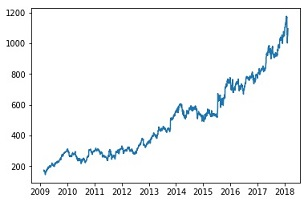
\includegraphics{./figures/1.jpg}
\caption{}
\end{figure}

\begin{itemize}
\tightlist
\item
  Output: Prediction Price at the current day based on historical data
\item
  Optional output: Suggest Buy/Sell/Hold
\end{itemize}

\subsection{Problem Statement}\label{problem-statement}

\begin{itemize}
\tightlist
\item
  The main task here is to predict the current(t) based on historical
  data(t-1, t-2, ...)
\item
  I suggest 2 different approaches:

  \begin{itemize}
  \tightlist
  \item
    Traditional supervised machine learning methods(Regressions)
  \item
    A specific machine learning method for time series forecasting(ARIMA
    model)
  \end{itemize}
\item
  Subproblems have to be considered that time series data:

  \begin{itemize}
  \tightlist
  \item
    Are very noisy
  \item
    Are different from tabular data that each data point related to each
    other
  \item
    Contain time-dependent structures:

    \begin{itemize}
    \tightlist
    \item
      Level: the average value in the series
    \item
      Trend: global increasing or decreasing
    \item
      Seasonalities: repeating pattern of the series
    \end{itemize}
  \end{itemize}
\end{itemize}

\subsection{Metrics}\label{metrics}

\begin{itemize}
\tightlist
\item
  Evalute models based on the error produced by predictions and
  observations
\item
  RMSE(Root Mean Squared Error) definition:
  \[RMSE = \sqrt{\frac{\sum_{t \in N}(y_t - \hat{y}_t)^2}{N}}\]
\item
  Reasons to choose RMSE:

  \begin{itemize}
  \tightlist
  \item
    Squaring error to have positive values
  \item
    Putting more weight on large errors
  \end{itemize}
\item
  Cons of choosing RMSE:

  \begin{itemize}
  \tightlist
  \item
    Our data may have many outliers that affect the perfomance
    evaluation
  \end{itemize}
\end{itemize}

\section{Analysis}\label{analysis}

\subsection{Data Exploration}\label{data-exploration}

\begin{itemize}
\tightlist
\item
  Input data:

  \begin{itemize}
  \tightlist
  \item
    Datetime and Adjusted Close
  \item
    4 symbols: AAPL, GOOG, XOM, GLD
  \item
    Datetime range: 8 years(from 01-01-2010 to 31-12-2017) \\
    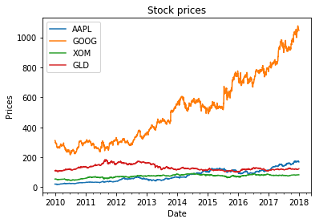
\includegraphics{./figures/2.jpg}
  \end{itemize}
\item
  Data preprocessing: Normalization \\ \\
  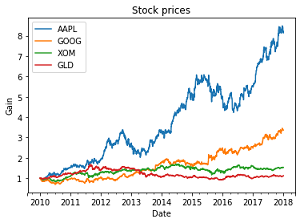
\includegraphics{./figures/3.jpg}
\end{itemize}

Observations in normalized series: + GOOG has a constantly increasing in
trend + AAPL has a strong increase and fluctuation + XOM and GLD have
the same pattern which trend components are low + So I choose 3 typical
series for Price Predicting Model: AAPL, GOOG, XOM

\subsection{Exploratory Visualization}\label{exploratory-visualization}

\begin{itemize}
\item
  Global statistic:

  \emph{Mean, Standard deviation, Median, Sum}
\end{itemize}

\begin{longtable}[]{@{}ccccc@{}}
\toprule
\textbf{Symbol} & \textbf{Mean} & \textbf{Std} & \textbf{Median} &
\textbf{Sum}\tabularnewline
\midrule
\endhead
AAPL & 3.743462 & 1.968410 & 3.252886 & 10938.396687\tabularnewline
GOOG & 1.658303 & 0.722951 & 1.656681 & 4845.562630\tabularnewline
XOM & 1.356500 & 0.197727 & 1.402289 & 3963.693878\tabularnewline
GLD & 1.187735 & 0.176200 & 1.124818 & 3470.562110\tabularnewline
\bottomrule
\end{longtable}

\begin{verbatim}
Observations:
    + AAPL has the highest variance and mean value
    + XOM and GLD has the lowest variance as visualization
    
\end{verbatim}

\begin{itemize}
\tightlist
\item
  Rolling Statistic

  \begin{itemize}
  \tightlist
  \item
    Bollinger Band Analysis:
  \item
    Parameter: \texttt{windowsize=20,\ Year=2015}: Indicates the trend
    is resting or variating at the current time
  \end{itemize}
\end{itemize}

\[ Upper\_band = Rolling\_mean + 2*std \]
\[ Lower\_band = Rolling\_mean - 2*std \] \\
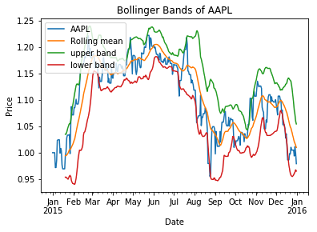
\includegraphics{./figures/4.jpg} 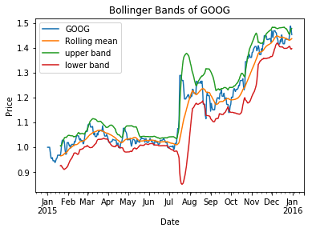
\includegraphics{./figures/5.jpg} \\
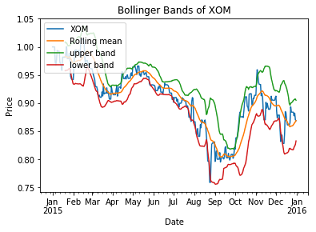
\includegraphics{./figures/6.jpg} 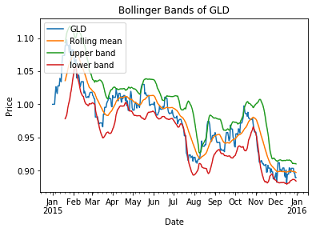
\includegraphics{./figures/7.jpg}

\begin{itemize}
\item
  Lagged order analysis: Time-series data have a special property that
  current datapoint(t) strongly corellated to previous historical
  datapoints(t-1, t-2, ..., t-n) \\
  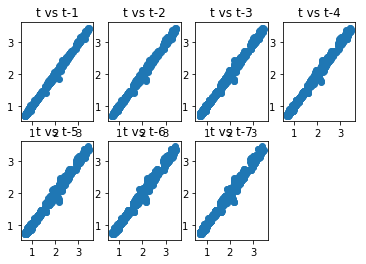
\includegraphics{./figures/8.jpg}

  \begin{itemize}
  \item
    AAPL \\
    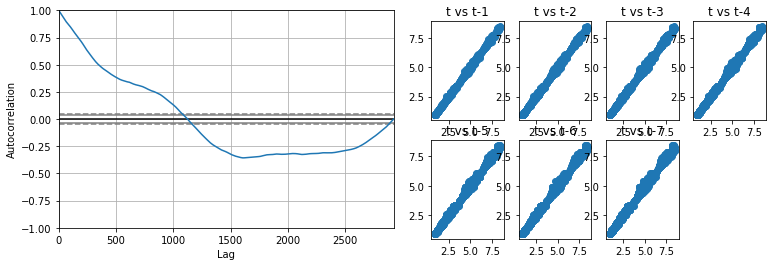
\includegraphics{./figures/19.jpg}
  \item
    GOOG \\
    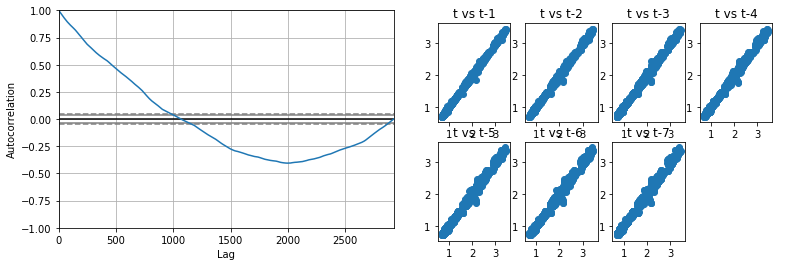
\includegraphics{./figures/22.jpg}
  \item
    XOM \\ 
    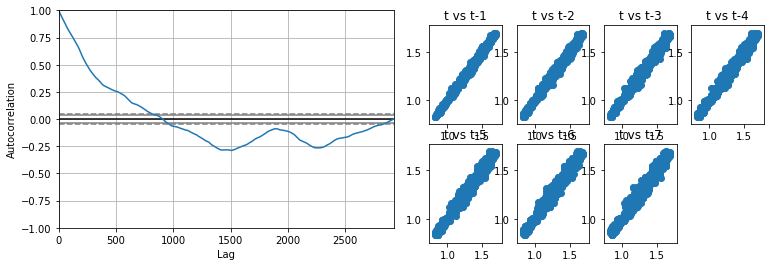
\includegraphics{./figures/25.jpg}
  \end{itemize}
\end{itemize}

\subsection{Algorithms and Techniques}\label{algorithms-and-techniques}

\subsubsection{Linear Regression
Approach}\label{linear-regression-approach}

\paragraph{Definition}\label{definition-1}

\begin{itemize}
\item
  Multiple Linear Regression model
  \[y = m + a_1*x_1 + a_2*x_2 + ... + a_n*x_n\]

  \begin{itemize}
  \tightlist
  \item
    m: intercept
  \item
    a\_n: parameters of feature n
  \item
    x\_n: feature n
  \item
    model parameters: (m, a\_1, a\_2, ..., a\_n)
  \end{itemize}
\item
  Fitting model

  \emph{Example} \[y = m + a_0*x\] \\
  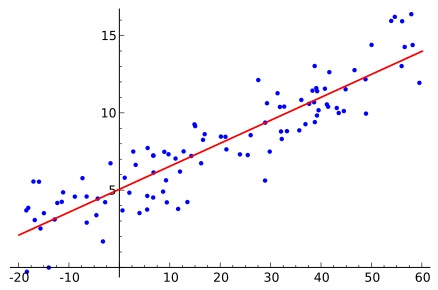
\includegraphics{./figures/30.jpg}
\end{itemize}

\paragraph{Feature engineering for Linear
Regression}\label{feature-engineering-for-linear-regression}

\begin{itemize}
\tightlist
\item
  For time series Regression, create lagged values as new features
  \[lag(n) = f(t-n) \] \emph{Example}: lagged values with n = 7
\end{itemize}

\begin{longtable}[]{@{}ccccccccc@{}}
\toprule
\textbf{Dates} & \textbf{t} & \textbf{t-1} & \textbf{t-2} & \textbf{t-3}
& \textbf{t-4} & \textbf{t-5} & \textbf{t-6} &
\textbf{t-7}\tabularnewline
\midrule
\endhead
2011-01-08 & 1.020005 & 1.020005 & 1.015140 & 1.007810 & 0.996310 &
1.000000 & 1.00000 & 1.00000\tabularnewline
2011-01-09 & 1.020005 & 1.020005 & 1.020005 & 1.015140 & 1.007810 &
0.996310 & 1.00000 & 1.00000\tabularnewline
2011-01-10 & 1.016315 & 1.020005 & 1.020005 & 1.020005 & 1.015140 &
1.007810 & 0.99631 & 1.00000\tabularnewline
2011-01-11 & 1.019293 & 1.016315 & 1.020005 & 1.020005 & 1.020005 &
1.015140 & 1.00781 & 0.99631\tabularnewline
2011-01-12 & 1.020716 & 1.019293 & 1.016315 & 1.020005 & 1.020005 &
1.020005 & 1.01514 & 1.00781\tabularnewline
\bottomrule
\end{longtable}

\begin{itemize}
\tightlist
\item
  Fit the model by n features(t-1, t-2, ..., t-n) to predict the current
  value(x(t)) \[x(t) = m + a_1*x(t-1) + a_2*x(t-2) + ... + a_2*x(t-2)\]
\item
  Perform grid search to find the optimal lag order n based on Root Mean
  Squared Error(RMSE)
\end{itemize}

\paragraph{Why Linear Regression ?}\label{why-linear-regression}

\begin{itemize}
\tightlist
\item
  Firstly, I choose Linear Regression as a baseline model to compare
  with the ARIMA model
\item
  The stock price prediction problem is similar to the regression
  problems(predict the current value based on historical data)
\end{itemize}

\subsubsection{ARIMA Approach}\label{arima-approach}

\paragraph{Definition}\label{definition-2}

\begin{itemize}
\tightlist
\item
  ARIMA stands for Autoregressive Integrated Moving Average (Alternative
  name: Box-Jenkins Model)
\item
  ARIMA is a forecasting technique that projects the future values of a
  series based on its own inertia
\item
  Its main application is short-term forecasting requiring at least 40
  historical data points
\item
  ARIMA works best when data:

  \begin{itemize}
  \tightlist
  \item
    Exhibits a stable or consistent pattern
  \item
    Have a minimum amount of outliers
  \end{itemize}
\end{itemize}

\paragraph{Models parameter}\label{models-parameter}

\begin{itemize}
\tightlist
\item
  ARIMA attempts to describe the movement in a stationary time series as
  a function of "autoregressive and moving avg"

  \begin{itemize}
  \tightlist
  \item
    AR(autoregressive)
  \item
    MA(moving avg)
  \end{itemize}
\item
  Autoregressive Models:
  \[X(t) = A(1)*X(t-1) + A(2)*X(t-2) +... + A(n)*X(t-n) + E(t)\]

  \begin{itemize}
  \tightlist
  \item
    X(t): the time-series
  \item
    X(t-n): time series lagged n
  \item
    A(n): autoregressive parameters
  \item
    E(t): the error term of the model
  \end{itemize}
\item
  Moving Average Models: \[X(t) = -B(1) * E(t-1) + E(t)\]

  \begin{itemize}
  \tightlist
  \item
    B(1): MA of order 1
  \item
    E(t): current error term
  \item
    E(t-1): error in the previous period
  \end{itemize}
\end{itemize}

\paragraph{Approach}\label{approach}

\begin{itemize}
\tightlist
\item
  Mixed ARIMA model is built on 3 parameters (p,d,q)

  \begin{itemize}
  \tightlist
  \item
    p: lag order
  \item
    d: degree of differencing
  \item
    q: size of moving average window(order of moving average)
  \end{itemize}
\item
  Perform grid search to find the optimal orders (p,d,q) based on Root
  mean squared error(RMSE)
\end{itemize}

\paragraph{Why ARIMA ?}\label{why-arima}

\begin{itemize}
\tightlist
\item
  ARIMA is a specific model for time-series analysis, I choose it to
  compare its performance versus the linear regression model
\item
  ARIMA has been proven that has a reliable accuracy, robustness over
  time-series prediction
\end{itemize}

\subsection{Benchmark}\label{benchmark}

\begin{itemize}
\tightlist
\item
  The Linear Regression model will be compared with the ARIMA model
\item
  Some Hypotheses I imply from Exploratory Visualization and Analysis:

  \begin{itemize}
  \tightlist
  \item
    Since AAPL time series data are strongly correlated, we can use more
    lagged values as input features thus the lagged order of ARIMA model
    would be set high
  \item
    Otherwise, XOM time series are not strongly correlated, the lagged
    order would be lower for this series.
  \item
    Though heavily affected by trend and fluctuation the ARIMA model
    tend to be less accurate in predicting AAPL and more accurate in
    predicting XOM series which is less affected by trend component and
    more stable
  \end{itemize}
\end{itemize}

\section{Methodology}\label{methodology}

\subsection{Data Preprocessing}\label{data-preprocessing}

\begin{itemize}
\item
  Normalization \[f(t) = \frac{f(t)}{f(0)}\] \\
  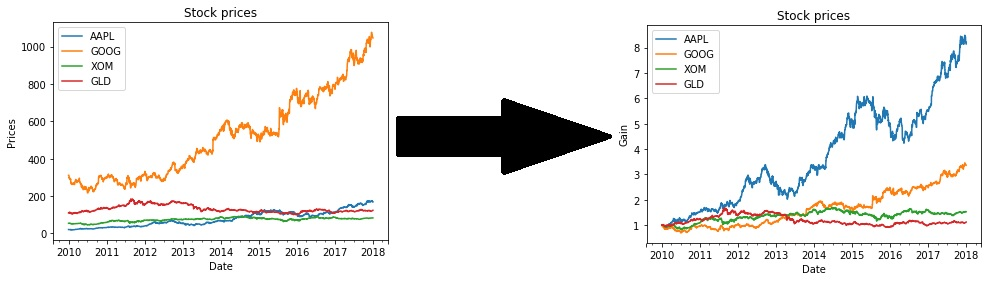
\includegraphics{./figures/13.jpg}
\item
  Why we need normalization

  \begin{itemize}
  \tightlist
  \item
    Compare multiple stocks easily in terms of variances, mean, median
    values
  \item
    Help with model convergence/stability
  \end{itemize}
\item
  Implementations

\begin{Shaded}
\begin{Highlighting}[]
\NormalTok{df }\OperatorTok{=}\NormalTok{ df}\OperatorTok{/}\NormalTok{df.iloc[}\DecValTok{0}\NormalTok{, :]}
\end{Highlighting}
\end{Shaded}
\end{itemize}

\subsection{Implementation}\label{implementation}

\subsubsection{Linear Regression}\label{linear-regression}

\begin{enumerate}
\def\labelenumi{\arabic{enumi}.}
\tightlist
\item
  Feature Engineering

  \begin{itemize}
  \tightlist
  \item
    Lagged values:

    \begin{itemize}
    \item
      We need lagged values(from x(t-1) to x(t-n)) as input features for
      the linear regression model
      \[x(t) = m + a_1*x(t-1) + a_2*x(t-2) + ... + a_2*x(t-2)\]
    \item
      How lagged features are created

\begin{Shaded}
\begin{Highlighting}[]
\ControlFlowTok{while}\NormalTok{ n }\OperatorTok{<}\NormalTok{ lagged_order:}
\NormalTok{    shift the series }\DecValTok{1}\NormalTok{ step }\KeywordTok{and}\NormalTok{ add a new feature }\ImportTok{as}\NormalTok{ x(t}\OperatorTok{-}\NormalTok{n)}
\NormalTok{Remove the empty entries of dataframe created by shifting}
\end{Highlighting}
\end{Shaded}
    \end{itemize}
  \item
    Examine correlation between lagged datapoints

    \begin{itemize}
    \tightlist
    \item
      Since my hypothesis is that we can predict the current in the
      series based on historical data, it is needed to check if the
      current value and previous values have a strong correlation.
    \item
      A strong correlation indicates that our linear regression model
      has prediction lower errors
    \item
      Thus, We can determine the lagged order suitable to generated as
      input features
    \end{itemize}

    Example \\
    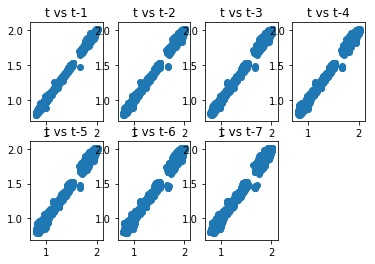
\includegraphics{./figures/14.jpg}
    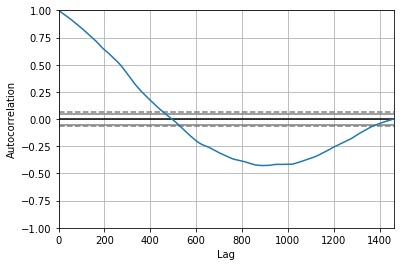
\includegraphics{./figures/15.jpg}
  \item
    Implementations

    \begin{itemize}
    \item
      Libraries

\begin{Shaded}
\begin{Highlighting}[]
\ImportTok{from}\NormalTok{ pandas.plotting }\ImportTok{import}\NormalTok{ autocorrelation_plot}
\end{Highlighting}
\end{Shaded}
    \item
      APIs

\begin{Shaded}
\begin{Highlighting}[]
\CommentTok{# Process the input time-series dataframe}
\CommentTok{# Return the dataframe corresponding to the lags-order}
\NormalTok{generate_lag(dataframe, lags)}

\CommentTok{# Plot the correlation of t vs (t-n)}
\NormalTok{plot_correlation(dataframe, lags)}
\end{Highlighting}
\end{Shaded}
    \end{itemize}
  \end{itemize}
\item
  Split data into trainning/validation/test set

  \begin{itemize}
  \tightlist
  \item
    Steps

    \begin{itemize}
    \tightlist
    \item
      Trainning set: train the model
    \item
      Validation set: validate the RMSE of the trained model, We choose
      the model which has lowest RMSE on validation
    \item
      Test set: Final evaluation of Linear Regression approach
    \end{itemize}

    Example \\
    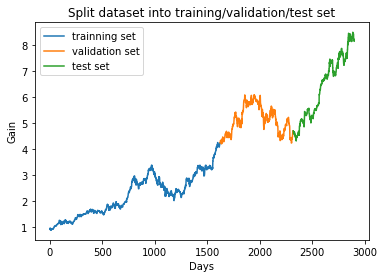
\includegraphics{./figures/16.jpg}
  \item
    Implementations

    \begin{itemize}
    \item
      APIs

\begin{Shaded}
\begin{Highlighting}[]
\CommentTok{# Split the dataset into 2 parts}
\CommentTok{# First part: 70% of the series}
\CommentTok{# Second part: 30% latter of the series}
\NormalTok{split_dataset(dataset, split_percentage}\OperatorTok{=}\FloatTok{0.7}\NormalTok{):}
\end{Highlighting}
\end{Shaded}
    \end{itemize}
  \end{itemize}
\item
  Perform grid search to find optimal parameters

  \begin{itemize}
  \tightlist
  \item
    Steps

    \begin{itemize}
    \item
      Examine which model has the lowest RMSE on validation set
    \item
      Hyper-parameters: (m, a\_1, a\_2, ..., a\_n) and the corresponding
      lagged order

\begin{Shaded}
\begin{Highlighting}[]
\ControlFlowTok{for}\NormalTok{ lag }\KeywordTok{in}\NormalTok{ lag_values:}
\NormalTok{    model }\OperatorTok{=}\NormalTok{ fit(trainning_set(X, y, lag))}
\NormalTok{    y_hat }\OperatorTok{=}\NormalTok{ model.predict(validation_set(X, lag))}
\NormalTok{    error }\OperatorTok{=}\NormalTok{ RMSE(y }\OperatorTok{-}\NormalTok{ y_hat)}
\NormalTok{    best_params }\OperatorTok{=}\NormalTok{ params }\ControlFlowTok{with}\NormalTok{ minimum error}
\ControlFlowTok{return}\NormalTok{ best_params}
\end{Highlighting}
\end{Shaded}
    \end{itemize}
  \item
    Implementations

    \begin{itemize}
    \item
      Libraries

\begin{Shaded}
\begin{Highlighting}[]
\ImportTok{from}\NormalTok{ sklearn.linear_model }\ImportTok{import}\NormalTok{ LinearRegression}
\end{Highlighting}
\end{Shaded}
    \item
      APIs

\begin{Shaded}
\begin{Highlighting}[]
\CommentTok{# Train a Linear Regression model with trainning set}
\CommentTok{# Return the predictions produced by testing set X}
\NormalTok{Linear_Regression_predict(train_X, train_y, test_X)}

\CommentTok{# Perform a grid search provided by trainning set and validation set}
\CommentTok{# Find the optimal lagged order within the range of lag_values}
\NormalTok{Linear_Regression_grid_search(train_X, train_y, valid_X, valid_y, lag_values)}
\end{Highlighting}
\end{Shaded}
    \end{itemize}
  \end{itemize}
\item
  Evaluate based on RMSE and visualization

  \begin{itemize}
  \tightlist
  \item
    Steps

    \begin{itemize}
    \tightlist
    \item
      Fit the best model with testing dataset
    \item
      Visualize and evaluate the model
    \end{itemize}

    Example \\
    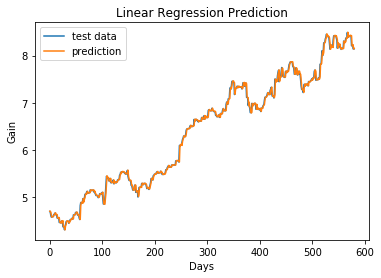
\includegraphics{./figures/17.jpg}
  \item
    Implimentations

    \begin{itemize}
    \item
      Libraries

\begin{Shaded}
\begin{Highlighting}[]
\ImportTok{from}\NormalTok{ sklearn.metrics }\ImportTok{import}\NormalTok{ mean_squared_error}
\ImportTok{from}\NormalTok{ math }\ImportTok{import}\NormalTok{ sqrt}
\end{Highlighting}
\end{Shaded}
    \item
      APIs

\begin{Shaded}
\begin{Highlighting}[]
\NormalTok{rmse }\OperatorTok{=}\NormalTok{ sqrt(mean_squared_error(validation_set, predictions))}
\end{Highlighting}
\end{Shaded}
    \end{itemize}
  \end{itemize}
\end{enumerate}

\subsubsection{ARIMA modeling}\label{arima-modeling}

\begin{enumerate}
\def\labelenumi{\arabic{enumi}.}
\tightlist
\item
  Split data into trainning/validation/test set

  \begin{itemize}
  \tightlist
  \item
    Steps

    \begin{itemize}
    \tightlist
    \item
      Trainning set: train the model
    \item
      Validation set: validate the RMSE of the trained model, We choose
      the model which has lowest RMSE on validation
    \item
      Test set: Final evaluation of Linear Regression approach
    \end{itemize}

    Example \\
    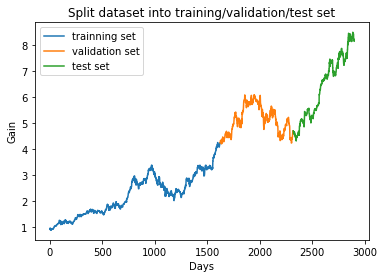
\includegraphics{./figures/16.jpg}
  \item
    Implimentations

    \begin{itemize}
    \item
      APIs

\begin{Shaded}
\begin{Highlighting}[]
\CommentTok{# Split the dataset into 2 parts}
\CommentTok{# First part: 70% of the series}
\CommentTok{# Second part: 30% latter of the series}
\NormalTok{split_dataset(dataset, split_percentage}\OperatorTok{=}\FloatTok{0.7}\NormalTok{):}
\end{Highlighting}
\end{Shaded}
    \end{itemize}
  \end{itemize}
\item
  Perform grid search to find optimal parameters

  \begin{itemize}
  \item
    Hyper-parameters: (p,d,q) of the model

\begin{Shaded}
\begin{Highlighting}[]
\ControlFlowTok{for}\NormalTok{ each (p,q,d) }\KeywordTok{in}\NormalTok{ order_values:}
\NormalTok{    model }\OperatorTok{=}\NormalTok{ fit(trainning_set(X, y, p, q, d))}
\NormalTok{    y_hat }\OperatorTok{=}\NormalTok{ model.predict(validation_set(X, p, q, d))}
\NormalTok{    error }\OperatorTok{=}\NormalTok{ RMSE(y }\OperatorTok{-}\NormalTok{ y_hat)}
\NormalTok{    best_params }\OperatorTok{=}\NormalTok{ params }\ControlFlowTok{with}\NormalTok{ minimum error}
\ControlFlowTok{return}\NormalTok{ best_params(p,q,d)}
\end{Highlighting}
\end{Shaded}
  \item
    Implimentations

    \begin{itemize}
    \item
      Libraries

\begin{Shaded}
\begin{Highlighting}[]
\ImportTok{from}\NormalTok{ statsmodels.tsa.arima_model }\ImportTok{import}\NormalTok{ ARIMA}
\end{Highlighting}
\end{Shaded}
    \item
      APIs

\begin{Shaded}
\begin{Highlighting}[]
\CommentTok{# Train a ARIMA model based on the trainning set with the correspondent order(p,d,q)}
\CommentTok{# Return predictions provided by testing set}
\NormalTok{train_ARIMA(train, test, orders)}

\CommentTok{# Perform a grid search provided by trainning set and testing set}
\CommentTok{# Find the optimal (p,d,q) order within the range of prvided p_values, d_values, q_values}
\NormalTok{grid_search_ARIMA(train, test, p_values, d_values, q_values)}
\end{Highlighting}
\end{Shaded}
    \end{itemize}
  \end{itemize}
\item
  Evaluate based on RMSE and visualization

  \begin{itemize}
  \tightlist
  \item
    Steps

    \begin{itemize}
    \tightlist
    \item
      Fit the best model with testing dataset
    \item
      Visualize and evaluate the model
    \end{itemize}

    Example \\
    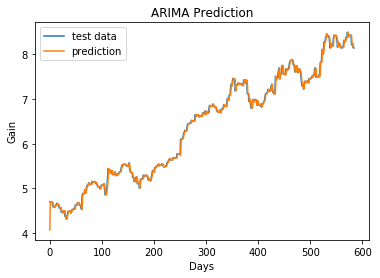
\includegraphics{./figures/18.jpg}
  \item
    Implimentations

    \begin{itemize}
    \item
      Libraries

\begin{Shaded}
\begin{Highlighting}[]
\ImportTok{from}\NormalTok{ sklearn.metrics }\ImportTok{import}\NormalTok{ mean_squared_error}
\ImportTok{from}\NormalTok{ math }\ImportTok{import}\NormalTok{ sqrt}
\end{Highlighting}
\end{Shaded}
    \item
      APIs

\begin{Shaded}
\begin{Highlighting}[]
\NormalTok{rmse }\OperatorTok{=}\NormalTok{ sqrt(mean_squared_error(validation_set, predictions))}
\end{Highlighting}
\end{Shaded}
    \end{itemize}
  \end{itemize}
\end{enumerate}

\subsection{Refinement}\label{refinement}

\begin{itemize}
\item
  Use the grid search to find the optimal parameters

\begin{Shaded}
\begin{Highlighting}[]
\ControlFlowTok{for}\NormalTok{ parameter }\KeywordTok{in}\NormalTok{ pre_defined_parameters:}
\NormalTok{    model }\OperatorTok{=}\NormalTok{ fit(trainning_set(X, y, parameter))}
\NormalTok{    y_hat }\OperatorTok{=}\NormalTok{ model.predict(validation_set(X))}
\NormalTok{    error }\OperatorTok{=}\NormalTok{ RMSE(y }\OperatorTok{-}\NormalTok{ y_hat)}
\NormalTok{    best_params }\OperatorTok{=}\NormalTok{ params }\ControlFlowTok{with}\NormalTok{ minimum error}
\ControlFlowTok{return}\NormalTok{ best_params}
\end{Highlighting}
\end{Shaded}
\item
  Linear Regression parameter: lagged order

  Example

\begin{verbatim}
lag order = 1 ----- rmse = 0.0681184299485
lag order = 2 ----- rmse = 0.0681223257362
lag order = 3 ----- rmse = 0.06815698406
lag order = 4 ----- rmse = 0.0681397973319
lag order = 5 ----- rmse = 0.0681668500541
lag order = 6 ----- rmse = 0.0680510359783
lag order = 7 ----- rmse = 0.0680368919466
lag order = 8 ----- rmse = 0.0681167632127
lag order = 9 ----- rmse = 0.0681144323532
lag order = 10 ----- rmse = 0.0682450179183
lag order = 11 ----- rmse = 0.0682020982234
lag order = 12 ----- rmse = 0.0682066932863
lag order = 13 ----- rmse = 0.068346349801
lag order = 14 ----- rmse = 0.0686007666681
lag order = 15 ----- rmse = 0.0685934882764
lag order = 16 ----- rmse = 0.0686576451934
lag order = 17 ----- rmse = 0.0686604377645
lag order = 18 ----- rmse = 0.0686682514038
lag order = 19 ----- rmse = 0.0687323543295
lag order = 20 ----- rmse = 0.0687804499171
\end{verbatim}

\begin{verbatim}
Best lag value: 7 which rmse: 0.068
\end{verbatim}
\item
  ARIMA parameter: corresponding (p,d,q)

  Example

\begin{verbatim}
(p,d,q) = (0, 0, 0) ----- rmse = 2.48364131894
(p,d,q) = (0, 0, 1) ----- rmse = 1.26650933811
(p,d,q) = (0, 1, 0) ----- rmse = 0.0679057555661
(p,d,q) = (0, 1, 1) ----- rmse = 0.0679954382993
(p,d,q) = (0, 1, 2) ----- rmse = 0.0680501205292
(p,d,q) = (0, 2, 0) ----- rmse = 0.0959062918676
(p,d,q) = (0, 2, 1) ----- rmse = 0.067961162253
(p,d,q) = (1, 0, 0) ----- rmse = 0.0678983071
(p,d,q) = (1, 1, 0) ----- rmse = 0.0679942677575
(p,d,q) = (1, 2, 0) ----- rmse = 0.0837961125124
(p,d,q) = (2, 1, 0) ----- rmse = 0.0680524002794
(p,d,q) = (2, 2, 0) ----- rmse = 0.0783914395604
(p,d,q) = (3, 1, 0) ----- rmse = 0.0680730399881
(p,d,q) = (3, 1, 1) ----- rmse = 0.0680880439241
(p,d,q) = (3, 2, 0) ----- rmse = 0.0759859093161
(p,d,q) = (4, 1, 0) ----- rmse = 0.0681052674349
(p,d,q) = (4, 1, 1) ----- rmse = 0.0680237050631
(p,d,q) = (4, 2, 0) ----- rmse = 0.0752259829098
(p,d,q) = (4, 2, 2) ----- rmse = 0.0680372743866
(p,d,q) = (5, 1, 0) ----- rmse = 0.0680484192109
(p,d,q) = (5, 1, 2) ----- rmse = 0.0680657372321
(p,d,q) = (5, 2, 0) ----- rmse = 0.0738266456692
(p,d,q) = (5, 2, 1) ----- rmse = 0.0681019681848
(p,d,q) = (5, 2, 2) ----- rmse = 0.068107805233
\end{verbatim}

\begin{verbatim}
Best order (p,d,q):  (1, 0, 0) which rmse = 0.068
\end{verbatim}
\end{itemize}

\section{Results}\label{results}

\subsection{Model Evaluation and
Validation}\label{model-evaluation-and-validation}

\subsubsection{AAPL}\label{aapl}

\begin{itemize}
\item
  Linear Regression model \\
  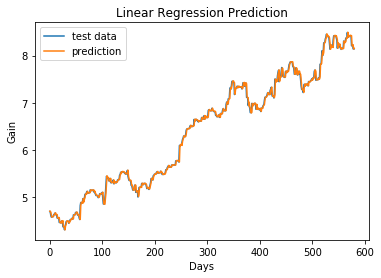
\includegraphics{./figures/20.jpg}

\begin{verbatim}
Best lag value: 7
Validation RMSE: 0.068
Test RMSE: 0.061
\end{verbatim}
\item
  ARIMA model \\
  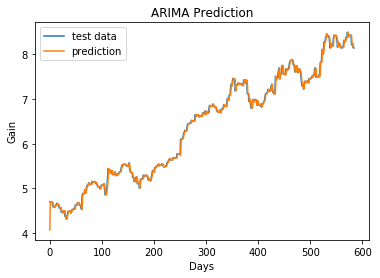
\includegraphics{./figures/21.jpg}

\begin{verbatim}
Best order (p,d,q): (1, 0, 0)
Validation RMSE: 0.068
Test RMSE: 0.066
\end{verbatim}
\item
  Evaluation

  \begin{itemize}
  \tightlist
  \item
    Both models work well on validation dataset
  \item
    For testing set, the Regression model seems to perform better
  \end{itemize}
\end{itemize}

\subsubsection{GOOG}\label{goog}

\begin{itemize}
\item
  Linear Regression model \\
  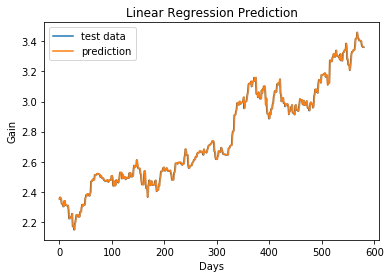
\includegraphics{./figures/23.jpg}

\begin{verbatim}
Best lag value: 1
Validation RMSE: 0.027
Test RMSE: 0.023
\end{verbatim}
\item
  ARIMA model \\
  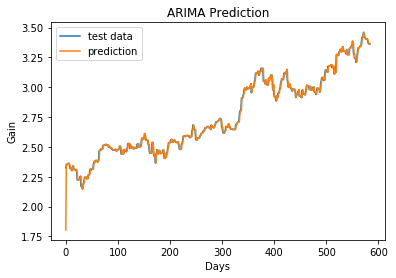
\includegraphics{./figures/24.jpg}

\begin{verbatim}
Best order (p,d,q): (0, 1, 0)
Validation RMSE: 0.027
Test RMSE: 0.031
\end{verbatim}
\item
  Evaluation

  \begin{itemize}
  \tightlist
  \item
    Both models work well on validation dataset
  \item
    For testing set, the ARIMA has a poor performance comapared to the
    Regression model
  \end{itemize}
\end{itemize}

\subsubsection{XOM}\label{xom}

\begin{itemize}
\item
  Linear Regression model \\
  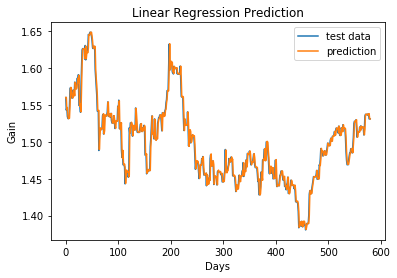
\includegraphics{./figures/26.jpg}

\begin{verbatim}
Best lag value: 4
Validation RMSE: 0.016
Test RMSE: 0.011
\end{verbatim}
\item
  ARIMA model \\
  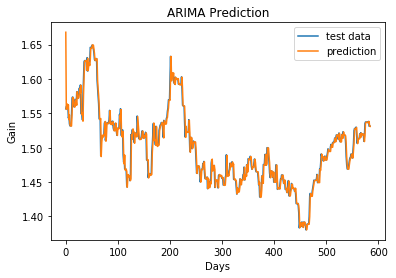
\includegraphics{./figures/27.jpg}

\begin{verbatim}
Best order (p,d,q): (4, 0, 2)
Validation RMSE: 0.016
Test RMSE: 0.012
\end{verbatim}
\item
  Evaluation

  \begin{itemize}
  \tightlist
  \item
    Both models work well on validation dataset
  \item
    For testing set, both models have the same performance with low
    errors
  \end{itemize}
\end{itemize}

\subsection{Robustness}\label{robustness}

\begin{itemize}
\item
  Test Robustness by predicting t+n days ahead(n=0,1,2,3,4,5,6,7) based
  on t-1,t-2...
\item
  Results

\begin{verbatim}
Predict t
Best lag value: 7, validation rmse: 0.068
Test RMSE: 0.060

Predict t + 1
Best lag value: 6, validation rmse: 0.096
Test RMSE: 0.086

Predict t + 2
Best lag value: 1, validation rmse: 0.117
Test RMSE: 0.106

Predict t + 3
Best lag value: 1, validation rmse: 0.135
Test RMSE: 0.124

Predict t + 4
Best lag value: 1, validation rmse: 0.151
Test RMSE: 0.141

Predict t + 5
Best lag value: 1, validation rmse: 0.164
Test RMSE: 0.156

Predict t + 6
Best lag value: 1, validation rmse: 0.176
Test RMSE: 0.168

Predict t + 7
Best lag value: 1, validation rmse: 0.185
Test RMSE: 0.182
\end{verbatim}
\item
  Explaination

  \begin{itemize}
  \tightlist
  \item
    RMSE in both validation and test set increasing
  \item
    Best lagged order reduced to 1
  \item
    We can imply that the model is not robust after predicting 2 days
    ahead
  \end{itemize}
\end{itemize}

\subsection{Justification}\label{justification}

\begin{itemize}
\tightlist
\item
  The Linear Regression model outperforms ARIMA model in nearly every
  cases
\item
  As prediction

  \begin{itemize}
  \tightlist
  \item
    The accuracy of ARIMA model is low on AAPL and high on XOM series
  \item
    Linear Regression model uses a high lagged order to predict
  \end{itemize}
\item
  Wrong hypothesis:

  \begin{itemize}
  \tightlist
  \item
    ARIMA model predicting XOM series needs complicated parameters
  \item
    ARIMA model predicting GOOG series has a low accuracy
  \end{itemize}
\end{itemize}

\section{Conclusion}\label{conclusion}

\subsection{Free-Form Visualization}\label{free-form-visualization} \\

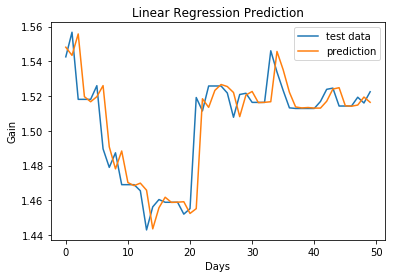
\includegraphics{./figures/28.jpg} 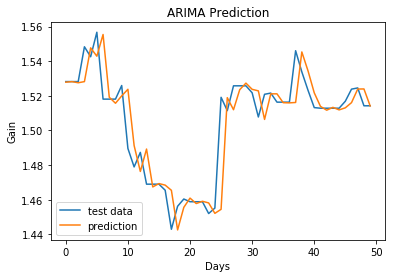
\includegraphics{./figures/29.jpg}

\begin{itemize}
\tightlist
\item
  If we look closely, the predicted series tend to be a lagged version
  of the actual series
\item
  Though we have a low RMSE result but I think it is not the best
  criteria to evaluate the stock predictor or time-series data in
  general
\item
  I guess it is useless to predict real stock data
\end{itemize}

\subsection{Reflection}\label{reflection}

\begin{itemize}
\tightlist
\item
  The ARIMA model accuracy is low which is interestingly unpredictable
\item
  The time required for training ARIMA model is high(\textasciitilde{}12
  hrs for grid searching optimization)
\item
  My hypothesis is that the ARIMA model is better than the Linear
  Regression model if there are no trend but the Linear Regression model
  seem to be strong enough to predict this nonconventional data
\item
  Based on the results, the ARIMA model works poorly with the
  time-series which have trend components like AAPL or GOOG stock data
\end{itemize}

\subsection{Improvement}\label{improvement}

\begin{itemize}
\tightlist
\item
  For ARIMA model we can remove the trend component before applying
  model fitting
\item
  We can remove the trend component by

  \begin{itemize}
  \item
    Subtract the time series by the previous value
    \[ x(t) = x(t) - x(t-1)\] \\
    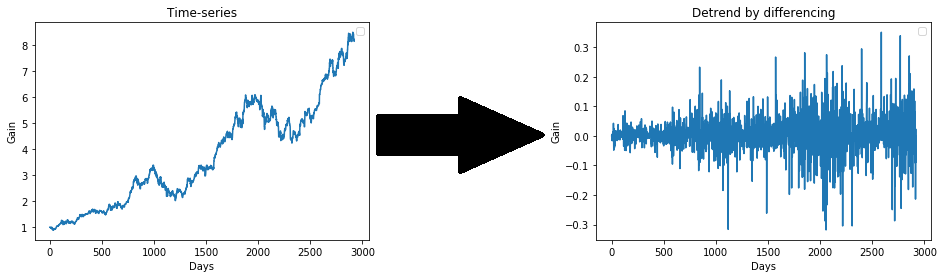
\includegraphics{./figures/31.jpg}
  \item
    Subtract the time series by the predicted value from a simple model

\begin{verbatim}
model = linearRegression()
predictions = model.fit(X)
X = X - predictions
\end{verbatim}

    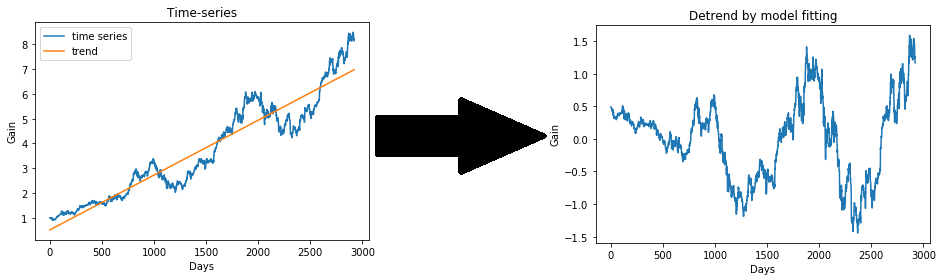
\includegraphics{./figures/32.jpg}
  \end{itemize}
\item
  Then used it as inputs for ARIMA models
\end{itemize}

\subsection{Challenges}\label{challenges}

\begin{itemize}
\tightlist
\item
  Time-series prediction is a non-trivial topic, I do not know how to
  approach it at the first time
\item
  RMSE or order error metrics are useless in predicting time-series data
\end{itemize}

\section{References}\label{references}

\begin{enumerate}
\def\labelenumi{\arabic{enumi}.}
\tightlist
\item
  \url{https://www.quora.com/What-is-ARIMA}
\item
  \url{https://www.quora.com/What-are-Bollinger-Bands}
\item
  \url{https://en.wikipedia.org/wiki/Linear_regression}
\item
  \href{https://www.udacity.com/course/machine-learning-for-trading--ud501}{Udacity
  - Machine Learning for Trading}
\item
  \href{https://stats.stackexchange.com/questions/84321/why-and-when-do-we-normalize}{https://stats.stackexchange.com/questions/84321/why-and-when-do-we-normalize-time-series-data}
\item
  \url{https://machinelearningmastery.com/time-series-trends-in-python/}
\end{enumerate}


    % Add a bibliography block to the postdoc
    
    
    
    \end{document}
